\chapter{Basics}

\section{JavaScript}
There are a few big advantages offered by \textbf{\gls{JS}}.\\ Maybe the biggest advantage is that it comes with the web browser, so everybody can run it by simply typing in an \gls{URL}. This offers great possibilities, since the users don't have to install any software package. The provided application is immediately ready to use once it was loaded.

Today \gls{JS} is the most used programming language world wide (Picture: \ref{fig:JS}). \gls{JS} first appeared in 1995, originally developed at Netscape by Brendan Eich it had a simple purpose, dynamically manipulating the HTML DOM in the browser.\\
At the same time a company called Sun worked on a programming language called Java, Netscape and Sun decided to work together and followed the idea of making LiveScript using Java Applets.  Netscape noticed that it would be good marketing to rename LiveScript to \gls{JS}. Since Java already had a growing community and was liked by many people, so Netscape took the chance and \gls{JS} was born.

However both language don't share a lot of things together, Java is a normal, static, and highly typed programming language, it runs on a virtual machine and needs to be compiled, whereas the single threaded \gls{JS} only runs in the browser and is script. Nevertheless they share the C related syntax and some similarities regarding naming conventions, both support object oriented programming.

The following analysis shall show why Java Script is in many ways superior for web development. Jeff Attwood the co-founder of the  computer programming question-and-answer website Stack Overflow and Stack Exchange once said "Any application that can be written in \gls{JS}, will eventually be written in JavaScript". \cite{HistoryJS1} \cite{HistoryJS2} \cite{HistoryJS3}

\begin{figure}[H]
	\centering
	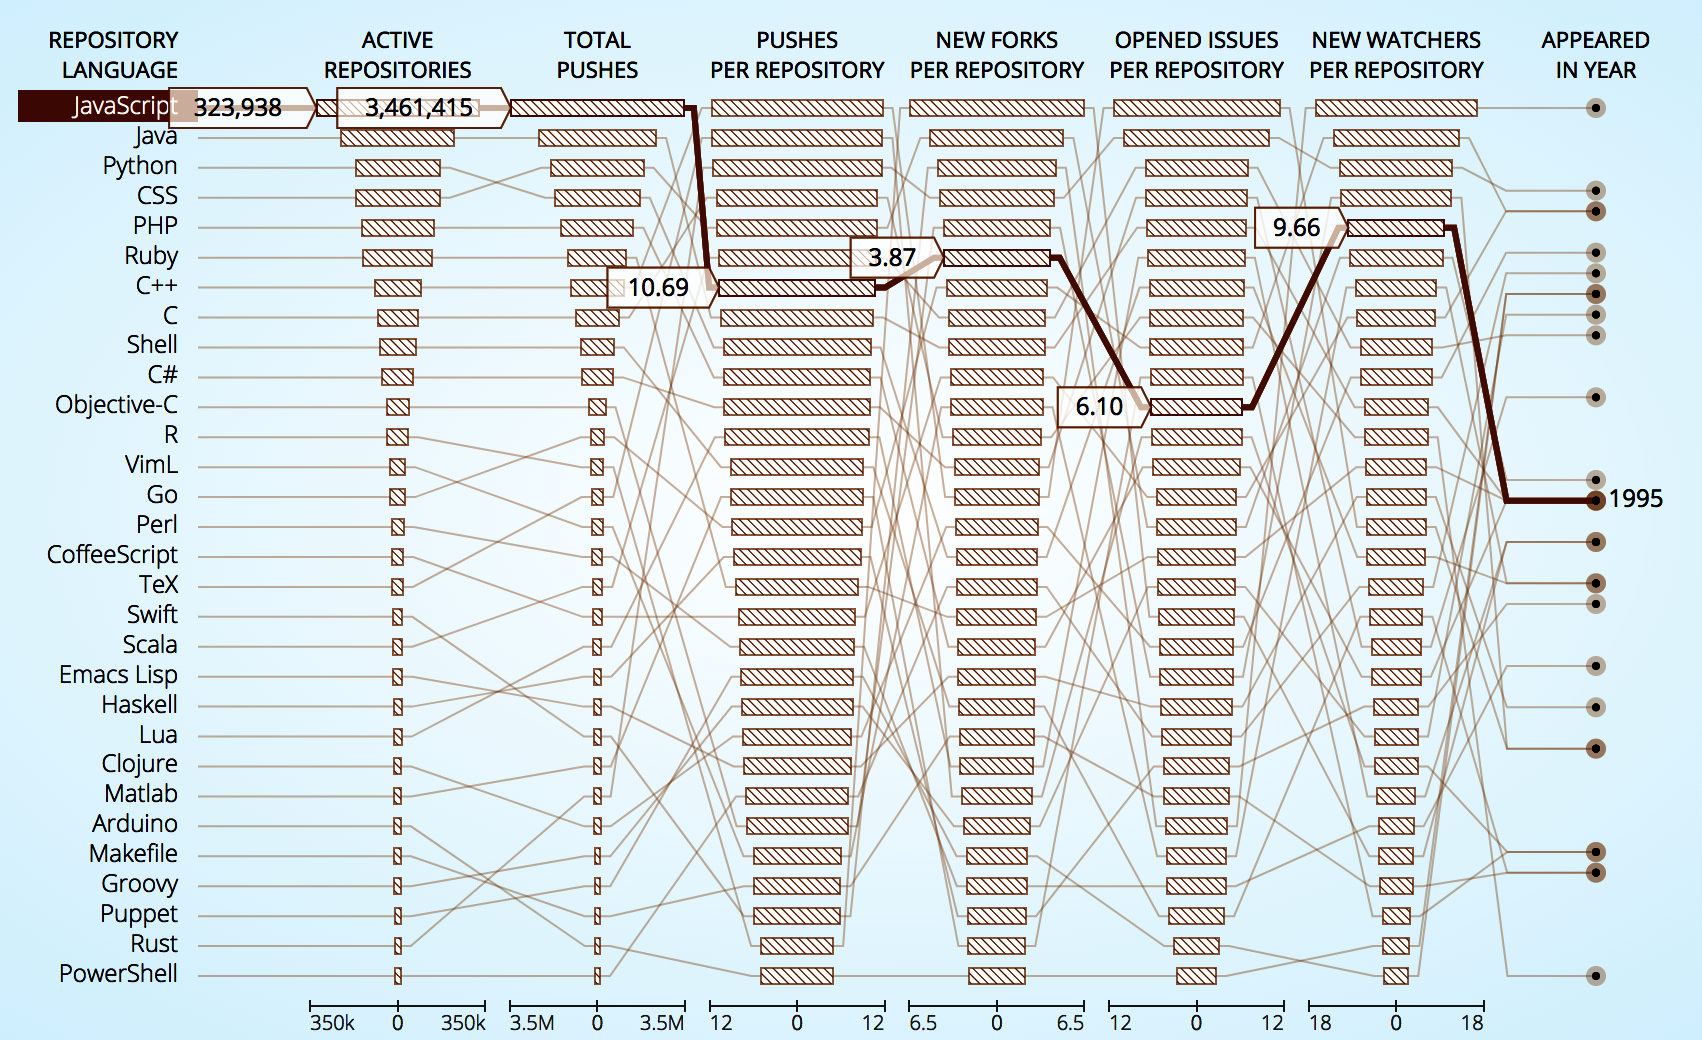
\includegraphics[scale=0.5]{bilder/grundlagen/jsUsage.png}
	\caption{Github Repositories Using JavaScript 2014} source:\cite{GitHut}
	\label{fig:JS}
\end{figure}

\newpage

\subsection{JavaScript Distributed Architectures}
Most modern web designs rely on they three-tier architecture. On the server side computing is done and data is stored in databases. The client fetches data from  server and makes it accessible. Often the user is able to change the data on client side. 

\begin{figure}[H]
	\centering
	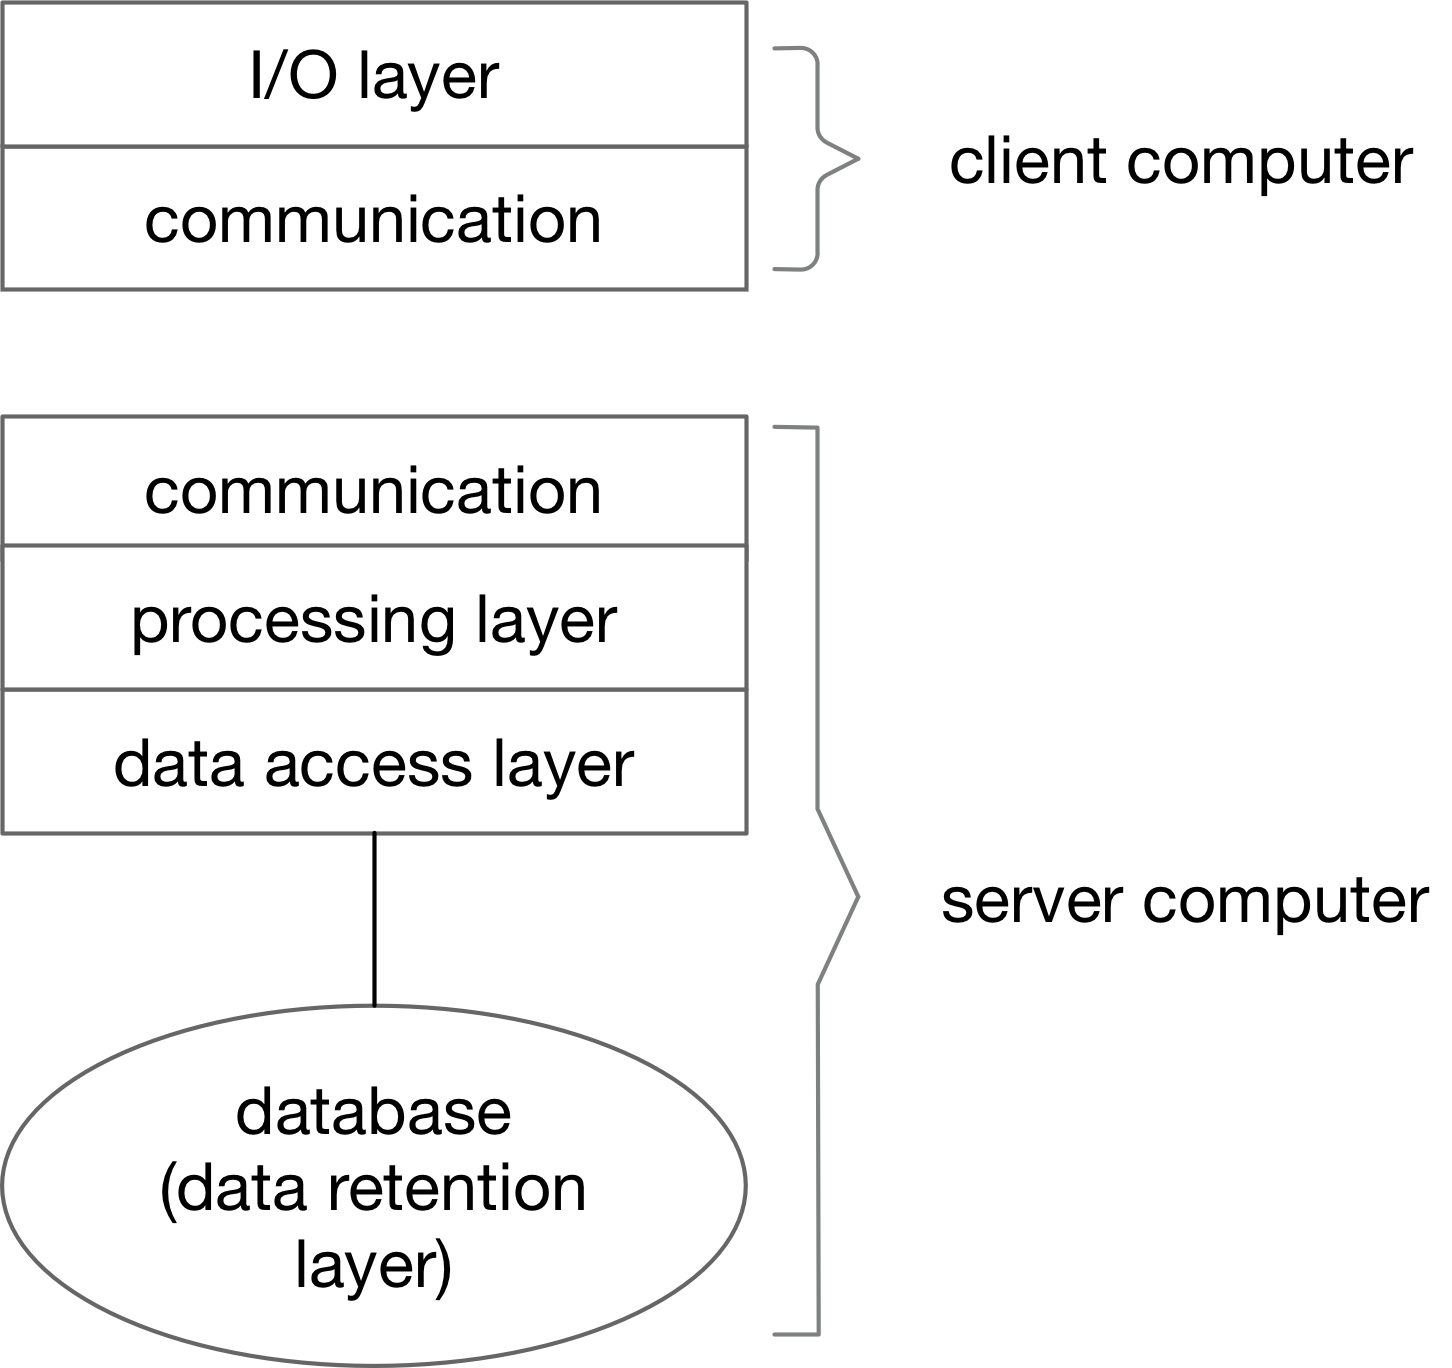
\includegraphics[scale=0.5]{bilder/grundlagen/Three-Tier.png}
	\caption{Three-Tier Architecture} source:\cite{TT}
	\label{fig:TT}
\end{figure}

For example deleting or adding a user, a request is sent to the server and a database change is done. For client side it facto mandatory to use \gls{JS}, but on server side  a large spectrum of languages is available, Java, CSharp, PHP, Ruby these are just the most famous one.

Once a user is added on client side, code is needed there in JavaScript. Same action needs to be implemented in a different language on server, 
therefore a second implementation is needed for the same action.
But the JavaScript ecosystem is undergoing rapid growth, with Node.js \gls{JS} is coming to the server and developers are now able to do whole applications in \gls{JS}.

That's big step, distributed systems that can use shared modules. It even affects the job market, front-end developers and back-end developers have been two separated jobs for over decades but now are one. People do not need to learn two languages anymore if they want to do full-stack web development, everything is covered with JavaScript.

\begin{figure}[H]
	\centering
	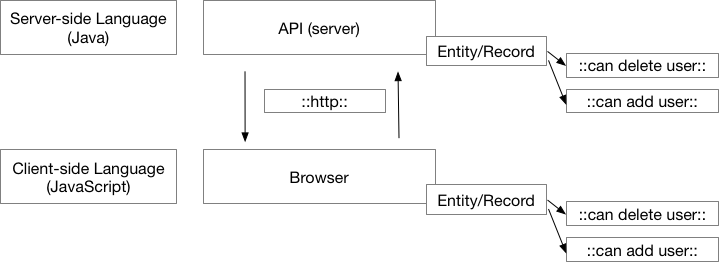
\includegraphics[scale=0.5]{bilder/grundlagen/Entity1.png}
	\caption{No Shared Modules} source:\cite{Distributed1}
	\label{fig:DS1}
\end{figure}

\begin{figure}[H]
	\centering
	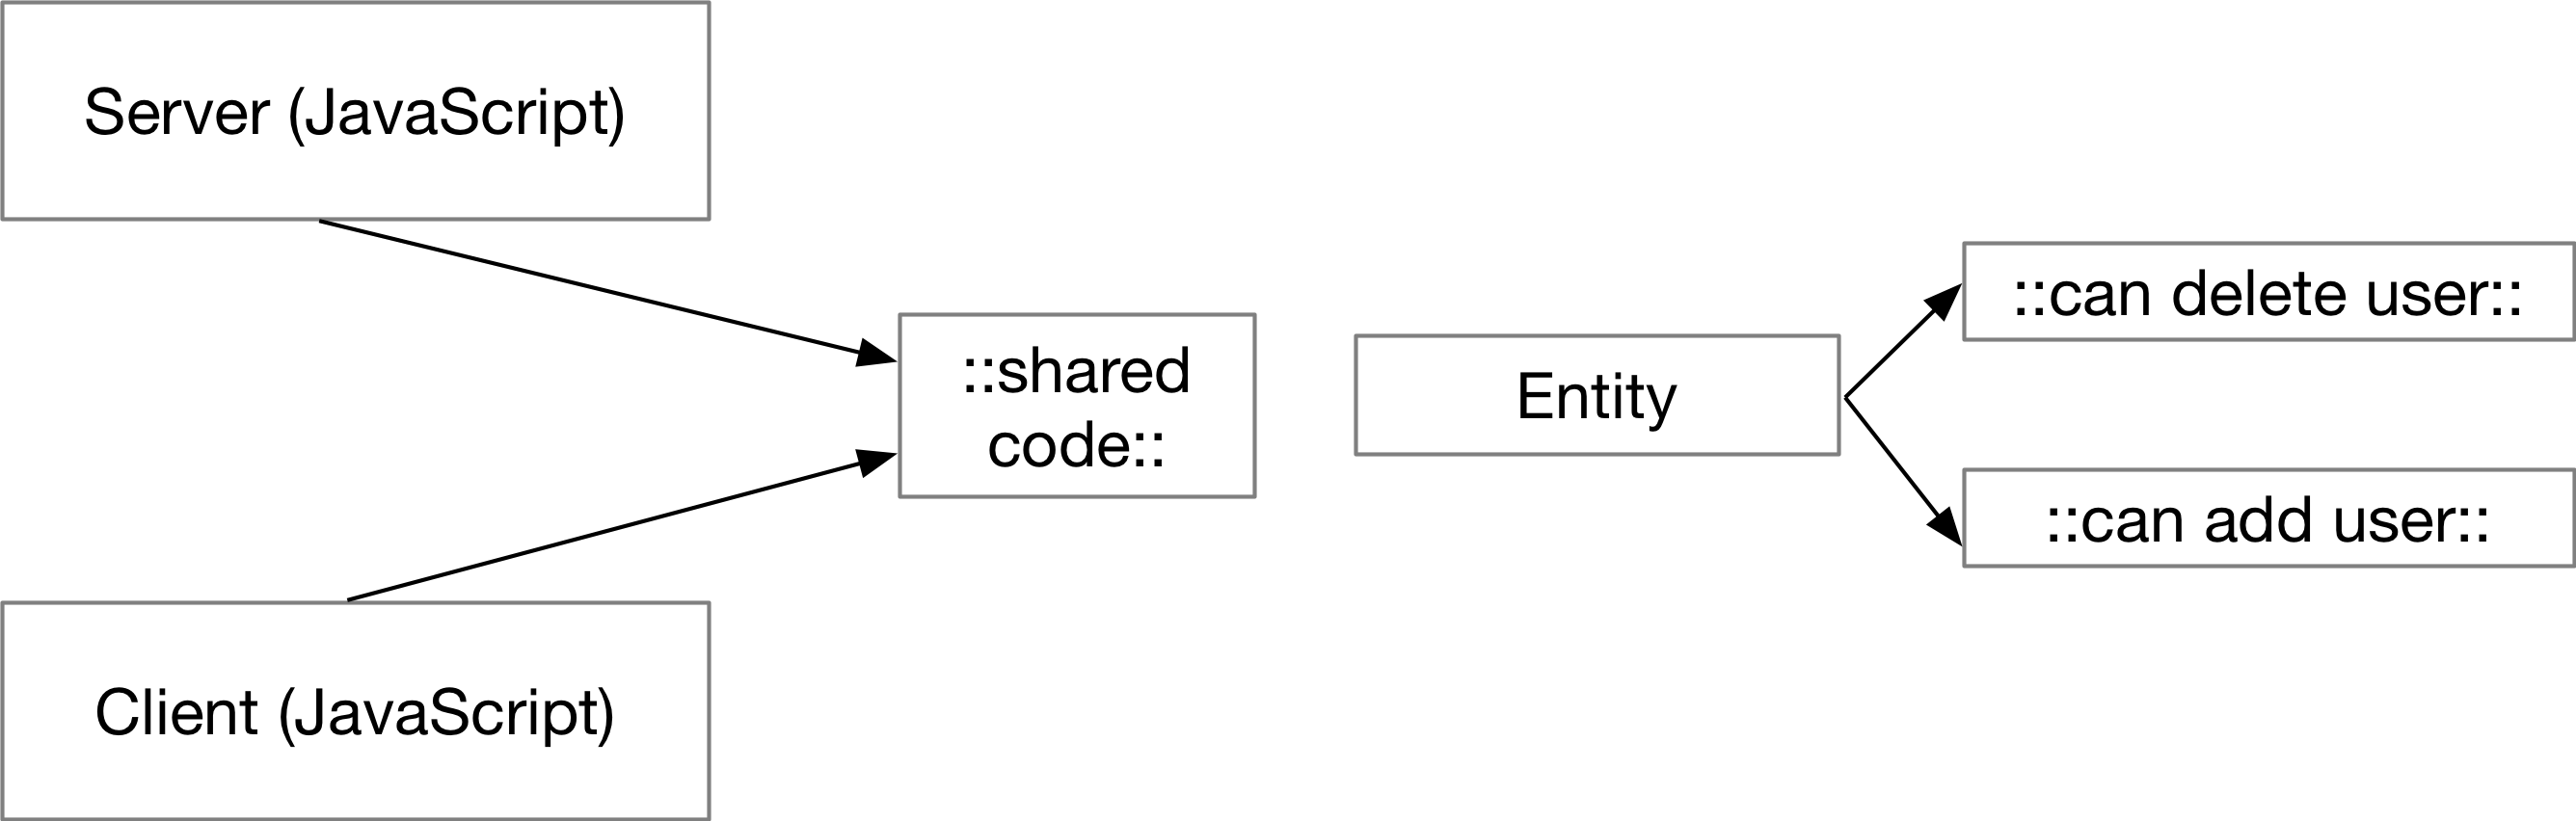
\includegraphics[scale=0.6]{bilder/grundlagen/Entity2.png}
	\caption{With Shared Modules} source:\cite{Distributed2}
	\label{fig:DS2}
\end{figure}


\subsection{Multi-Platform Support}

Deploying an application for the web browser is only one aspect of modern web development, often a separate implementation is needed for mobile devices or even desktop implementations. Two major operating systems are currently dominating the smart-phone market Android and IOS. 

Both support native App developing but that brings back the problem of having to implement the same functionality twice. Sure smart-phone Apps are different from browser based applications, starting with the touch event and ending up with totally different layouts. 

With JavaScript developers can take advantage of modern frameworks like React Native or Electron, which give the possibility to code in \gls{JS}, the JavaScript is communicating natively with implemented components written in Java on Android, Objective C on iOS, CSharp on Windows via an abstraction called bridge. Everytime \gls{JS} is called it forwards the call to the native code implementation, the response is passed back to the implemented abstraction \gls{JS}.

\begin{figure}[H]
	\centering
	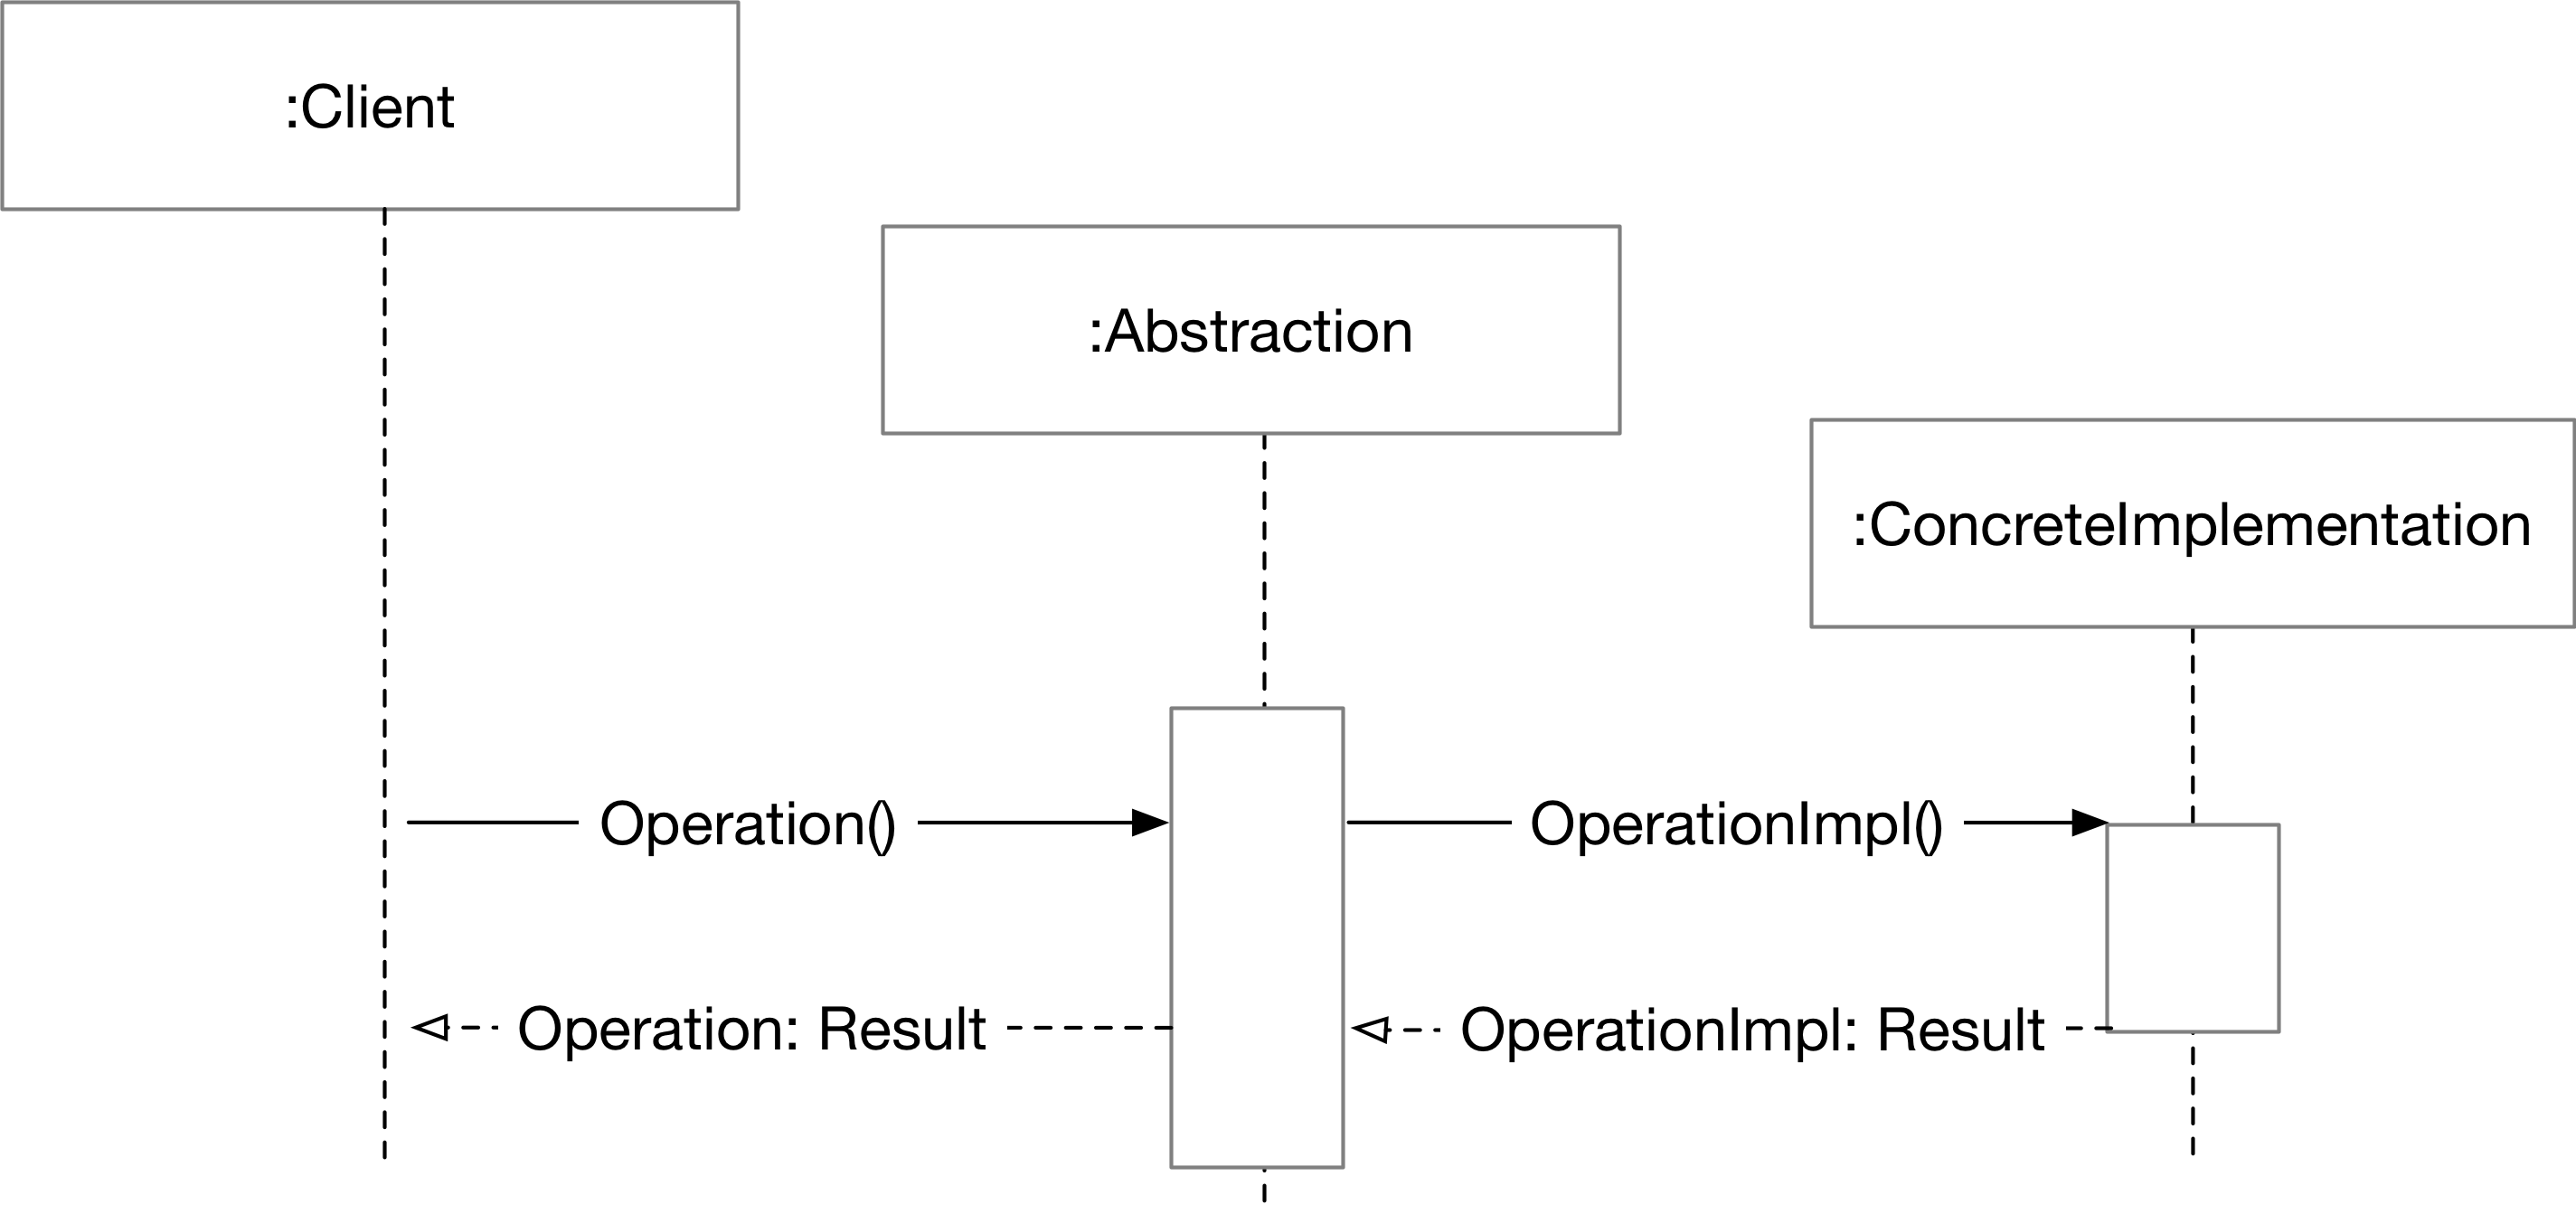
\includegraphics[scale=0.6]{bilder/grundlagen/BridgePattern.png}
	\caption{Bridge Pattern} source:\cite{GOLL}
	\label{fig:BP}
\end{figure}


\subsection{Single Threading and Concurrency}
The single treaded paradigm and non blocking architecture \gls{JS} is bond to, can be considered a weakness. Developing with JavaScript will generate errors and behavior that is perplexing . This section is about analyzing why \gls{JS} is relying on single threading and how it is still possible to add concurrency.

\gls{JS} was developed to manipulate the DOM, the DOM is a limited resource. Executing two pieces of code, asynchronously changing the same part of DOM would not be good. Given this single purpose it was decided to make JavaScript single threaded.

Actions that do not change the DOM should be able to run asynchronously. That makes sense, since fetching data from the server or reading a large list of files can take a lot of time and would block the browser, buttons would not be clickable anymore and any rendering would stop. 

How is it possible that JavaScript offers the opportunity to run code concurrently, even though it is single threaded? The following example how multi-threading is implemented in JavaScript.

Every time a function in \gls{JS} is called, it is put on the call stack. The result of that function is popped out from stack. The functions on stack are executed synchronously one after another.

\begin{figure}[H]
	\centering
	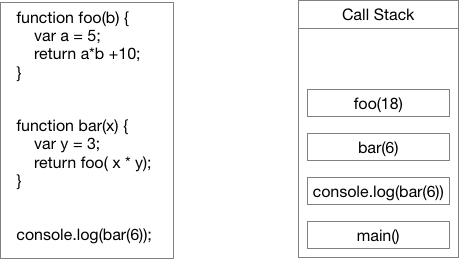
\includegraphics[scale=0.5]{bilder/grundlagen/CallStack.png}
	\caption{Call Stack} source:\cite{CallStack}
	\label{fig:CS}
\end{figure}

To execute code concurrently JavaScript needs to call the Web API, provided by the browser. The web browser is written in C++, so it fully supports multi-threading.

The Web API is called with a function that needs to be executed and a callback.
The callback tells what to do after the asynchronous function finished executing. It is mandatory to provide a callback with each asynchronous function.

Once the thread finished executing it passes the callback to as so called Callback Que. The Callback Que is a simple list with all callbacks that need to be executed. 

Further an event loop is responsible for checking if current stack is empty, if that's the case, the callback is put on stack and executed synchronously. The decoupling of the caller from the response allows for JavaScript to do other things while waiting for asynchronous operations to complete and their callbacks to fire. 

\begin{figure}[H]
	\centering
	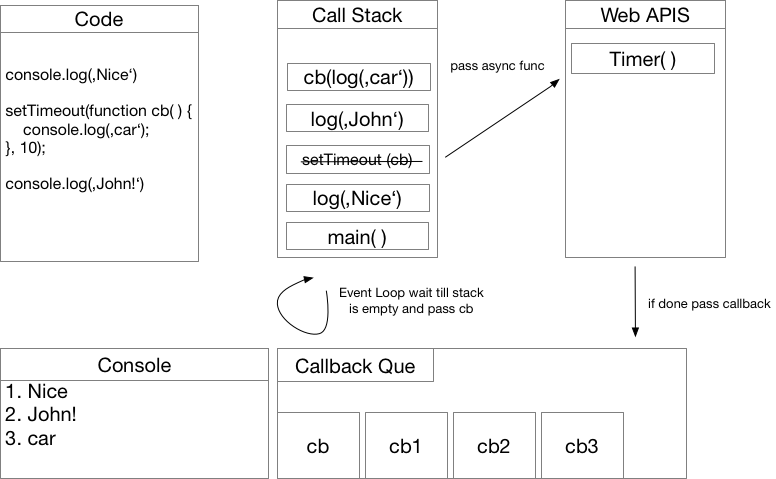
\includegraphics[scale=0.5]{bilder/grundlagen/Concurrency.png}
	\caption{Concurrency in JavaScript} source:\cite{Concurrency}
	\label{fig:CC}
\end{figure}

\subsection{Functional Programming Paradigm}
There is no need to use functional programming in JavaScript, since this is more a philosophy question and definitely nothing somebody needs to do when programming in JavaScript.Other ways of coding, like object oriented programming, are supported in JavaScript as well. This section shall explain what functional programming is and how it is implemented in JavaScript. No global variables or states are used in functional programming, the output of a function only depends on the input arguments.

\begin{figure}[H]
	\centering
	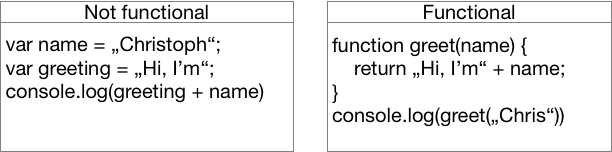
\includegraphics[scale=0.5]{bilder/grundlagen/fp.png}
	\caption{Imperative and Functional Programming} source:\cite{FP}
	\label{fig:FP}
\end{figure}

Another concept is the use of high-order functions. Giving the possibility to use functions as inputs and outputs. 


\begin{figure}[H]
	\centering
	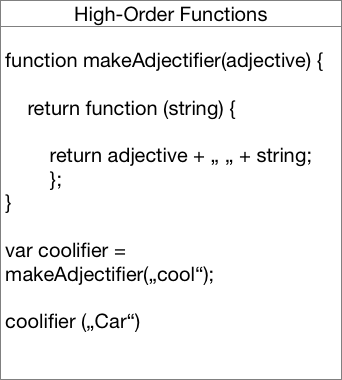
\includegraphics[scale=0.5]{bilder/grundlagen/fp1.png}
	\caption{High-Order Functions} source:\cite{HF}
	\label{fig:HF}
\end{figure}

Data mutation shall be avoided.

\begin{figure}[H]
	\centering
	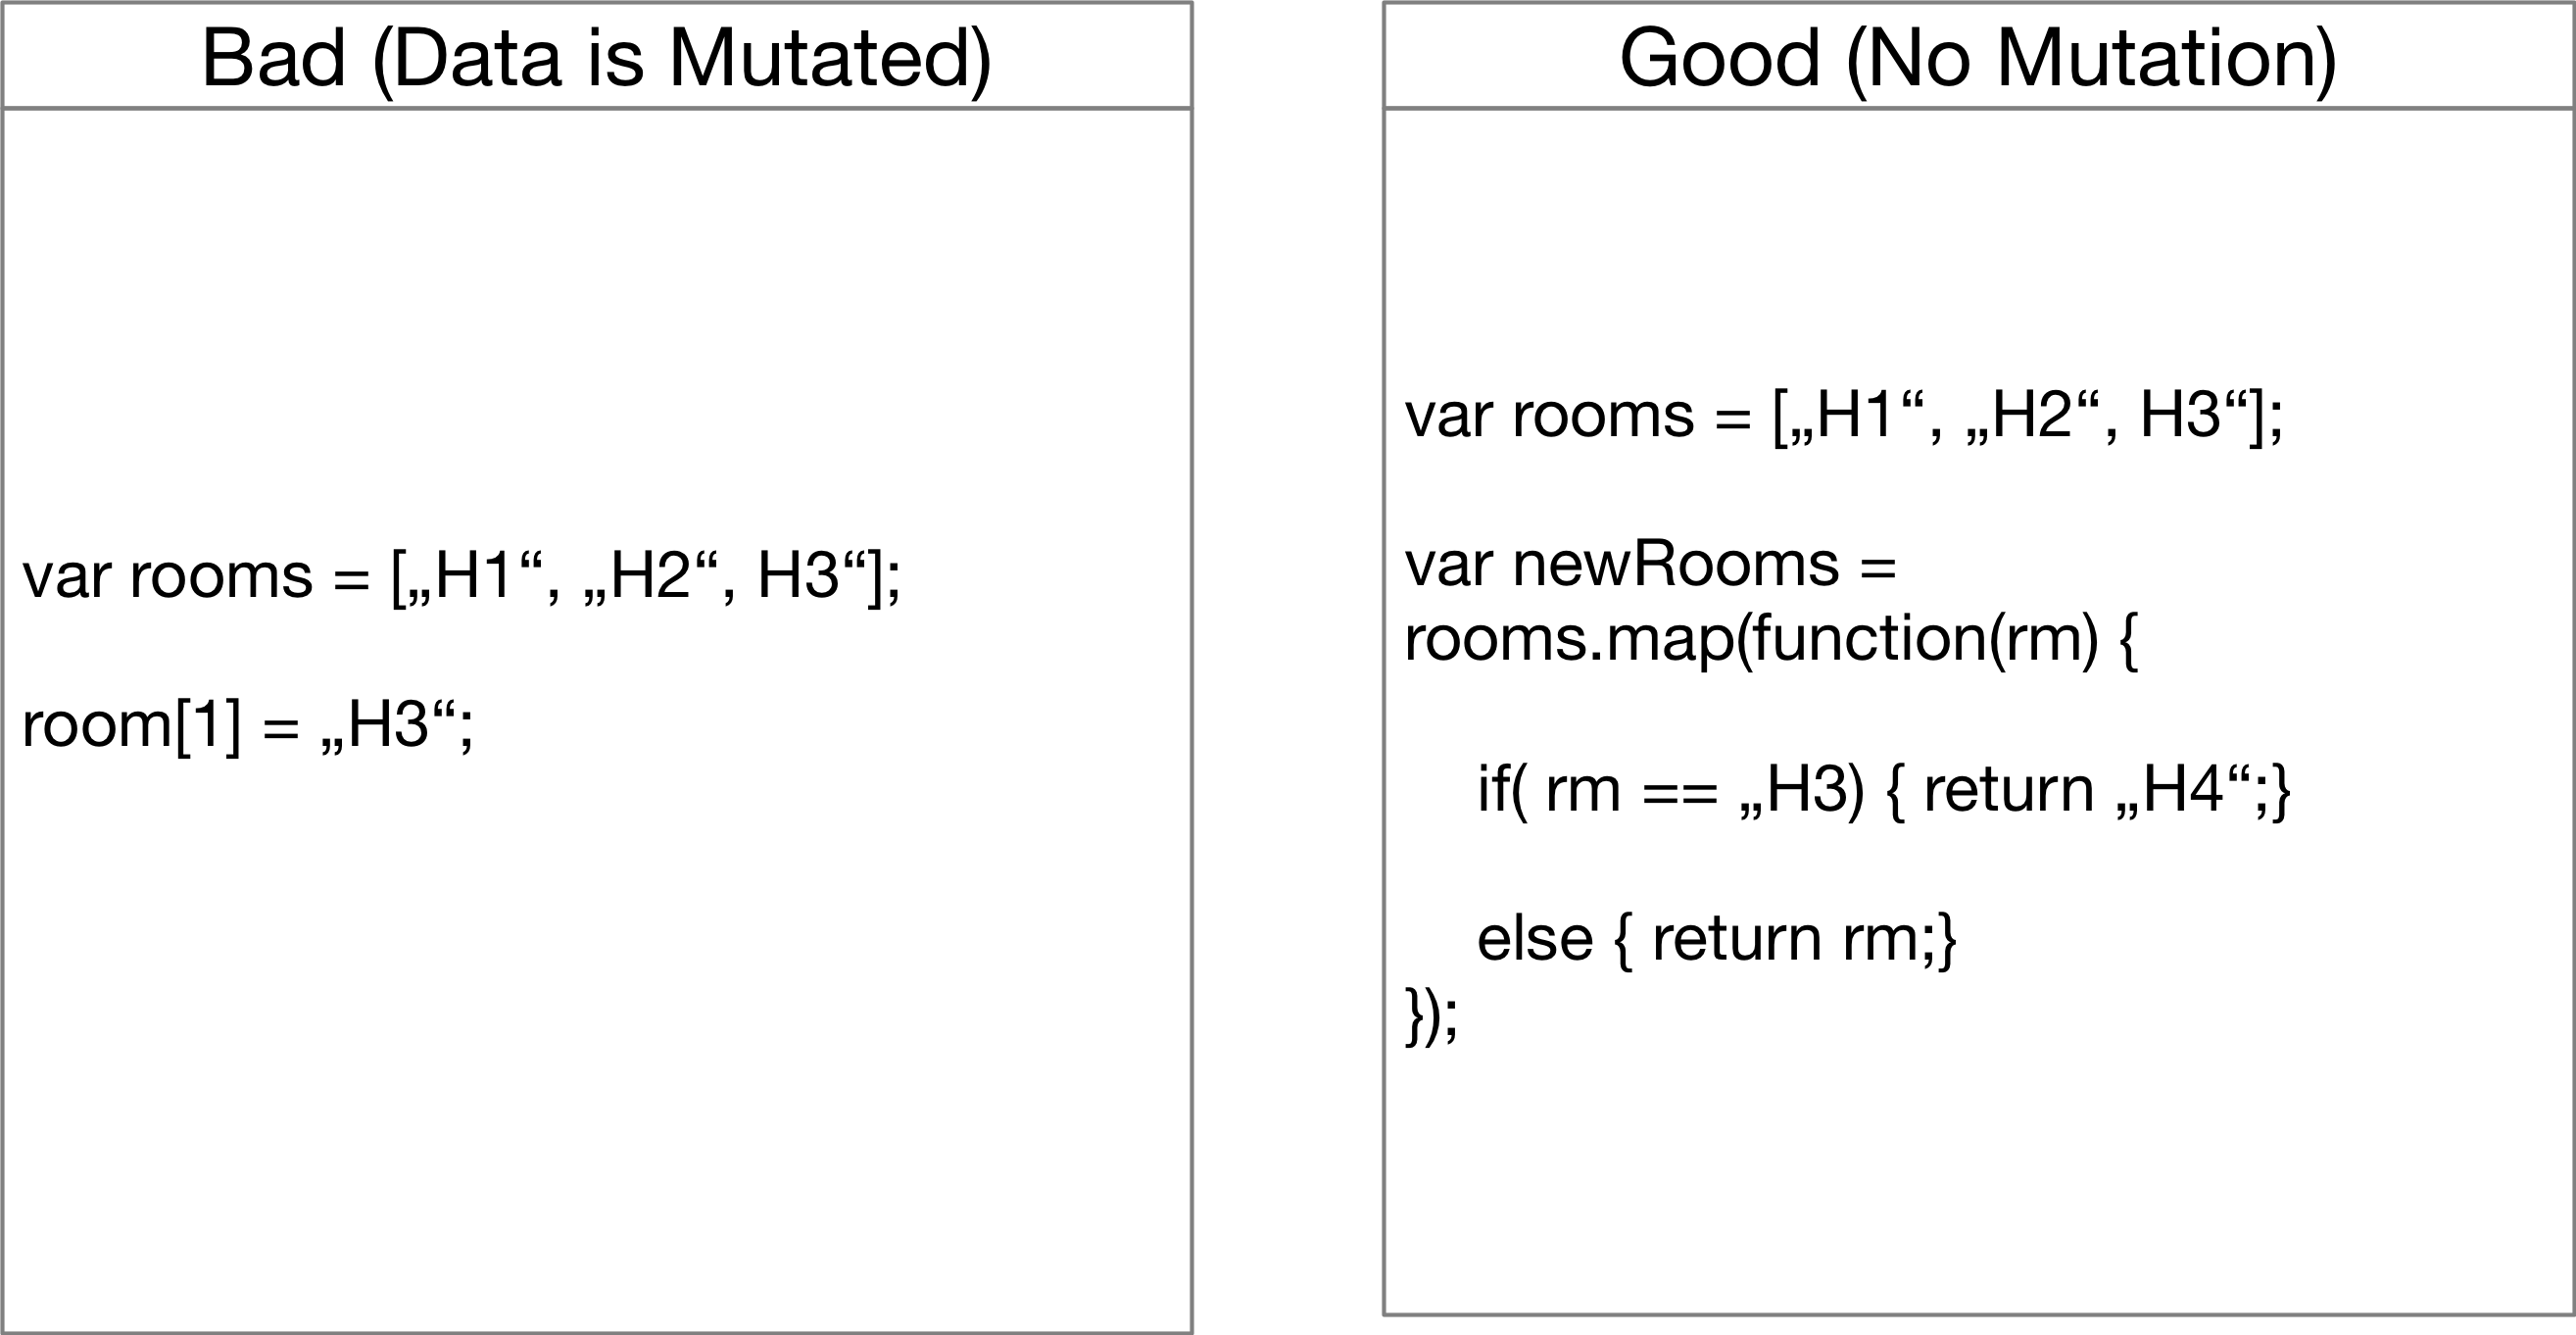
\includegraphics[scale=0.5]{bilder/grundlagen/fp2.png}
	\caption{Data Mutation} source:\cite{DM}
	\label{fig:DM}
\end{figure}

\newpage

\section{React}
Another key technology used in this project, is React. React is a JavaScript library for developing user interfaces. 

Back in 2011, Facebook noticed that it was getting hard to maintain their Application and to run it flawlessly, because of the growing number of features. Many people were hired and the team size expanded dramatically. With the growing team size it took longer to publish urgent updates, too many people were involved and concerns could not be separated in a satisfying manner.

A Facebook engineer called Jordan Walke decided to change that, in the same year he created FlaxJs, first prototype of React. Jordan was allowed to keep on working and created React (2012). 

A short time later Instagram was bought by Facebook and both companies agreed on using React as the new core technology for User Experience. Further they agreed on making React publicly available. 

In early 2013 at JS ConfUS, React became an open source project. Facebook CEO Mark Zuckerberg, speaking on the this conference said  "Our biggest mistake was betting too much on HTML5" and promised to provide better experiences with React.


\begin{figure}[H]
	\centering
	
\includegraphics[scale=0.1]{bilder/grundlagen/ReactLogo.png}
	\caption{The logo for the React open source JavaScript library} source:\cite{ReactLogo}
	\label{fig:RL}
\end{figure}

Currently React is getting more and more popular. A trend analysis, by Google shows that React is the leading modern User Experience JavaScript framework.

\begin{figure}[H]
	\centering
	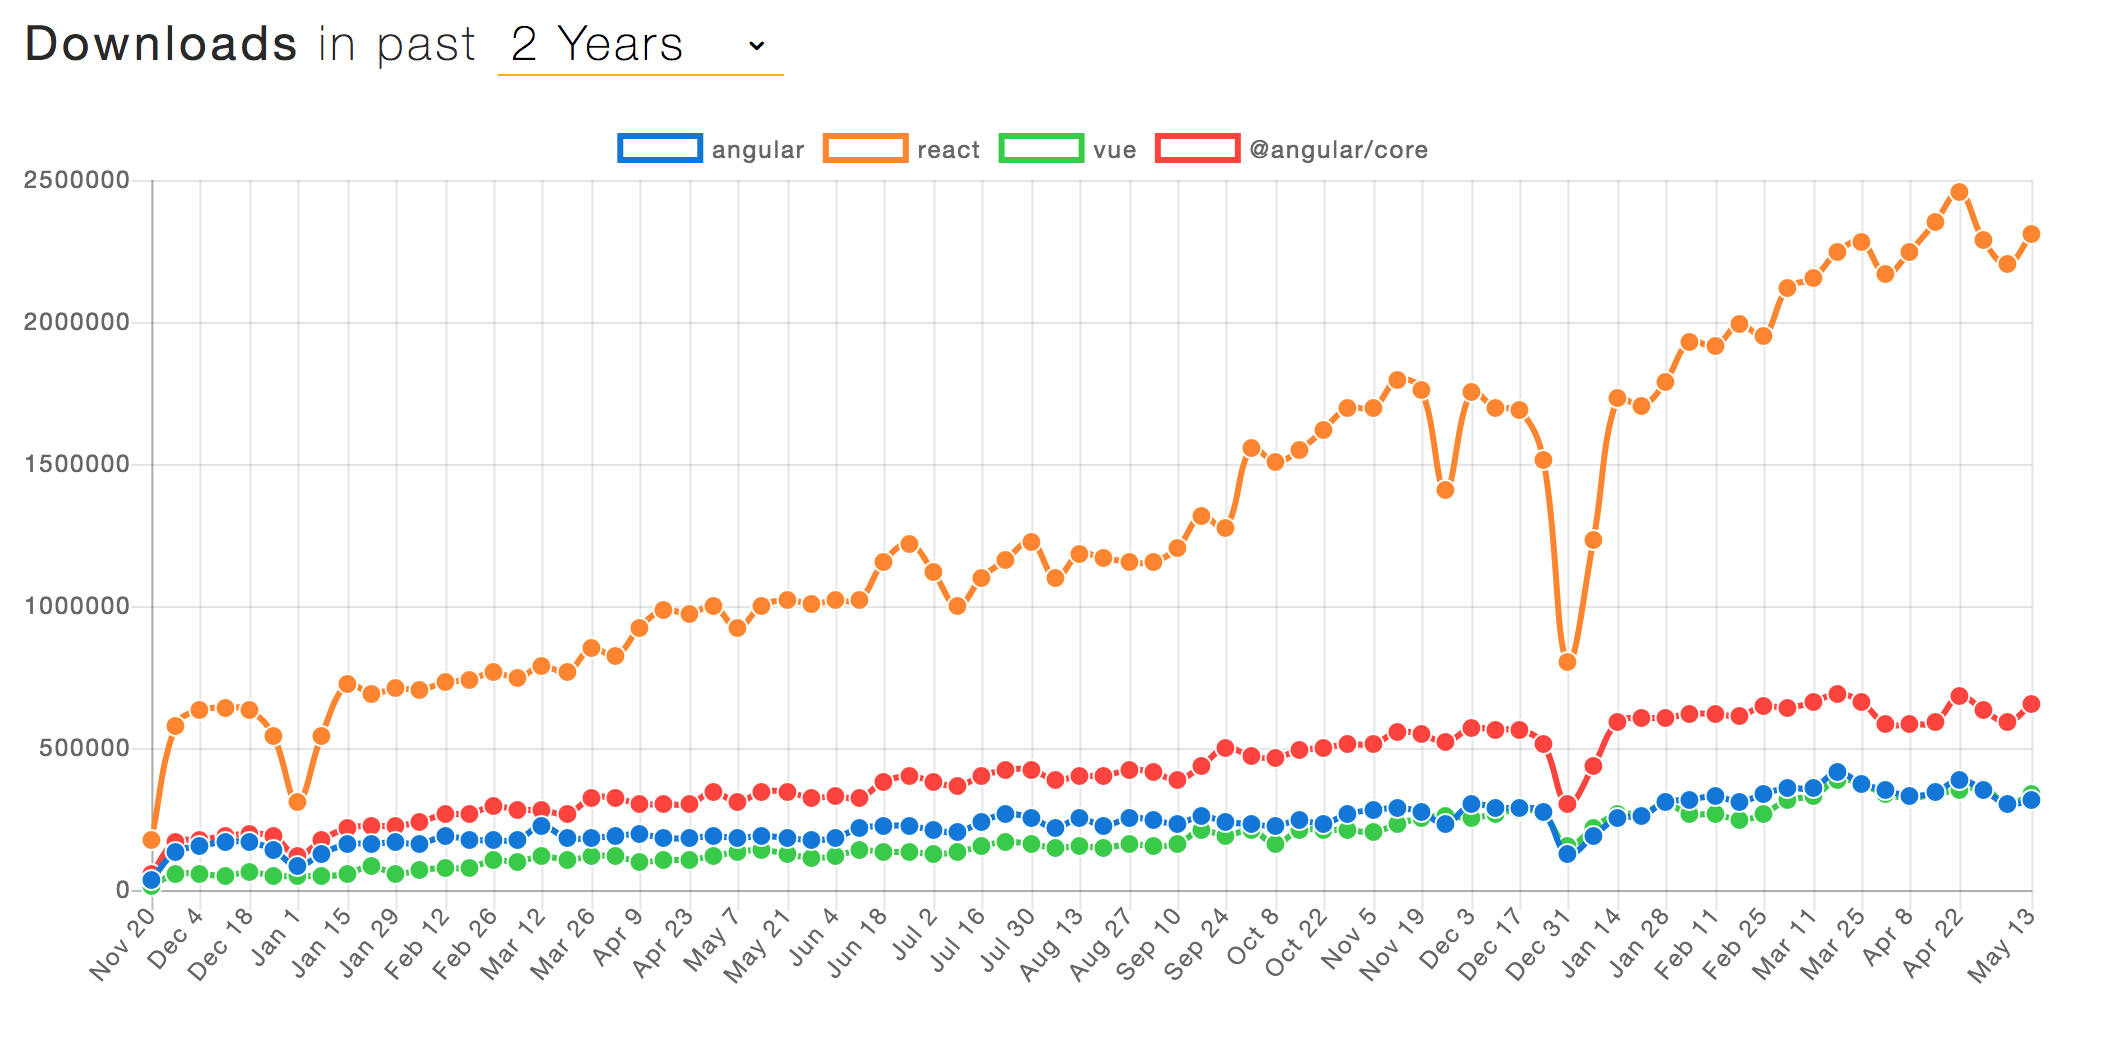
\includegraphics[scale=0.4]{bilder/grundlagen/ReactDownloads.png}
	\caption{Downloaded NPM Packages} source:\cite{NPM}
	\label{fig:JS}
\end{figure}


\subsection{Classic MVC Model}
For decades it was best practice to use the Model View Controller software architecture. The model stores the data presented in a view, in simple systems the model may contain business logic.

The model shall be independent of views and controllers. In case the model changes the controller may inform the views (passive Model). With an alternative active model implementation, the model informs the views. One model can have multiple views.
 
The view serves to present model data to user, there can be many views on the same model data. All views are updated in case of a model data change. A view may furthermore present interactive elements like buttons. 
 
Interaction with these elements creates events that usually are handled by the controller. The controller controls the model and view state, based on user input. It transforms events caused by user action into method calls of the model, the controller furthermore controls the state of view, for example activate or deactivate buttons.


\begin{figure}[H]
	\centering
	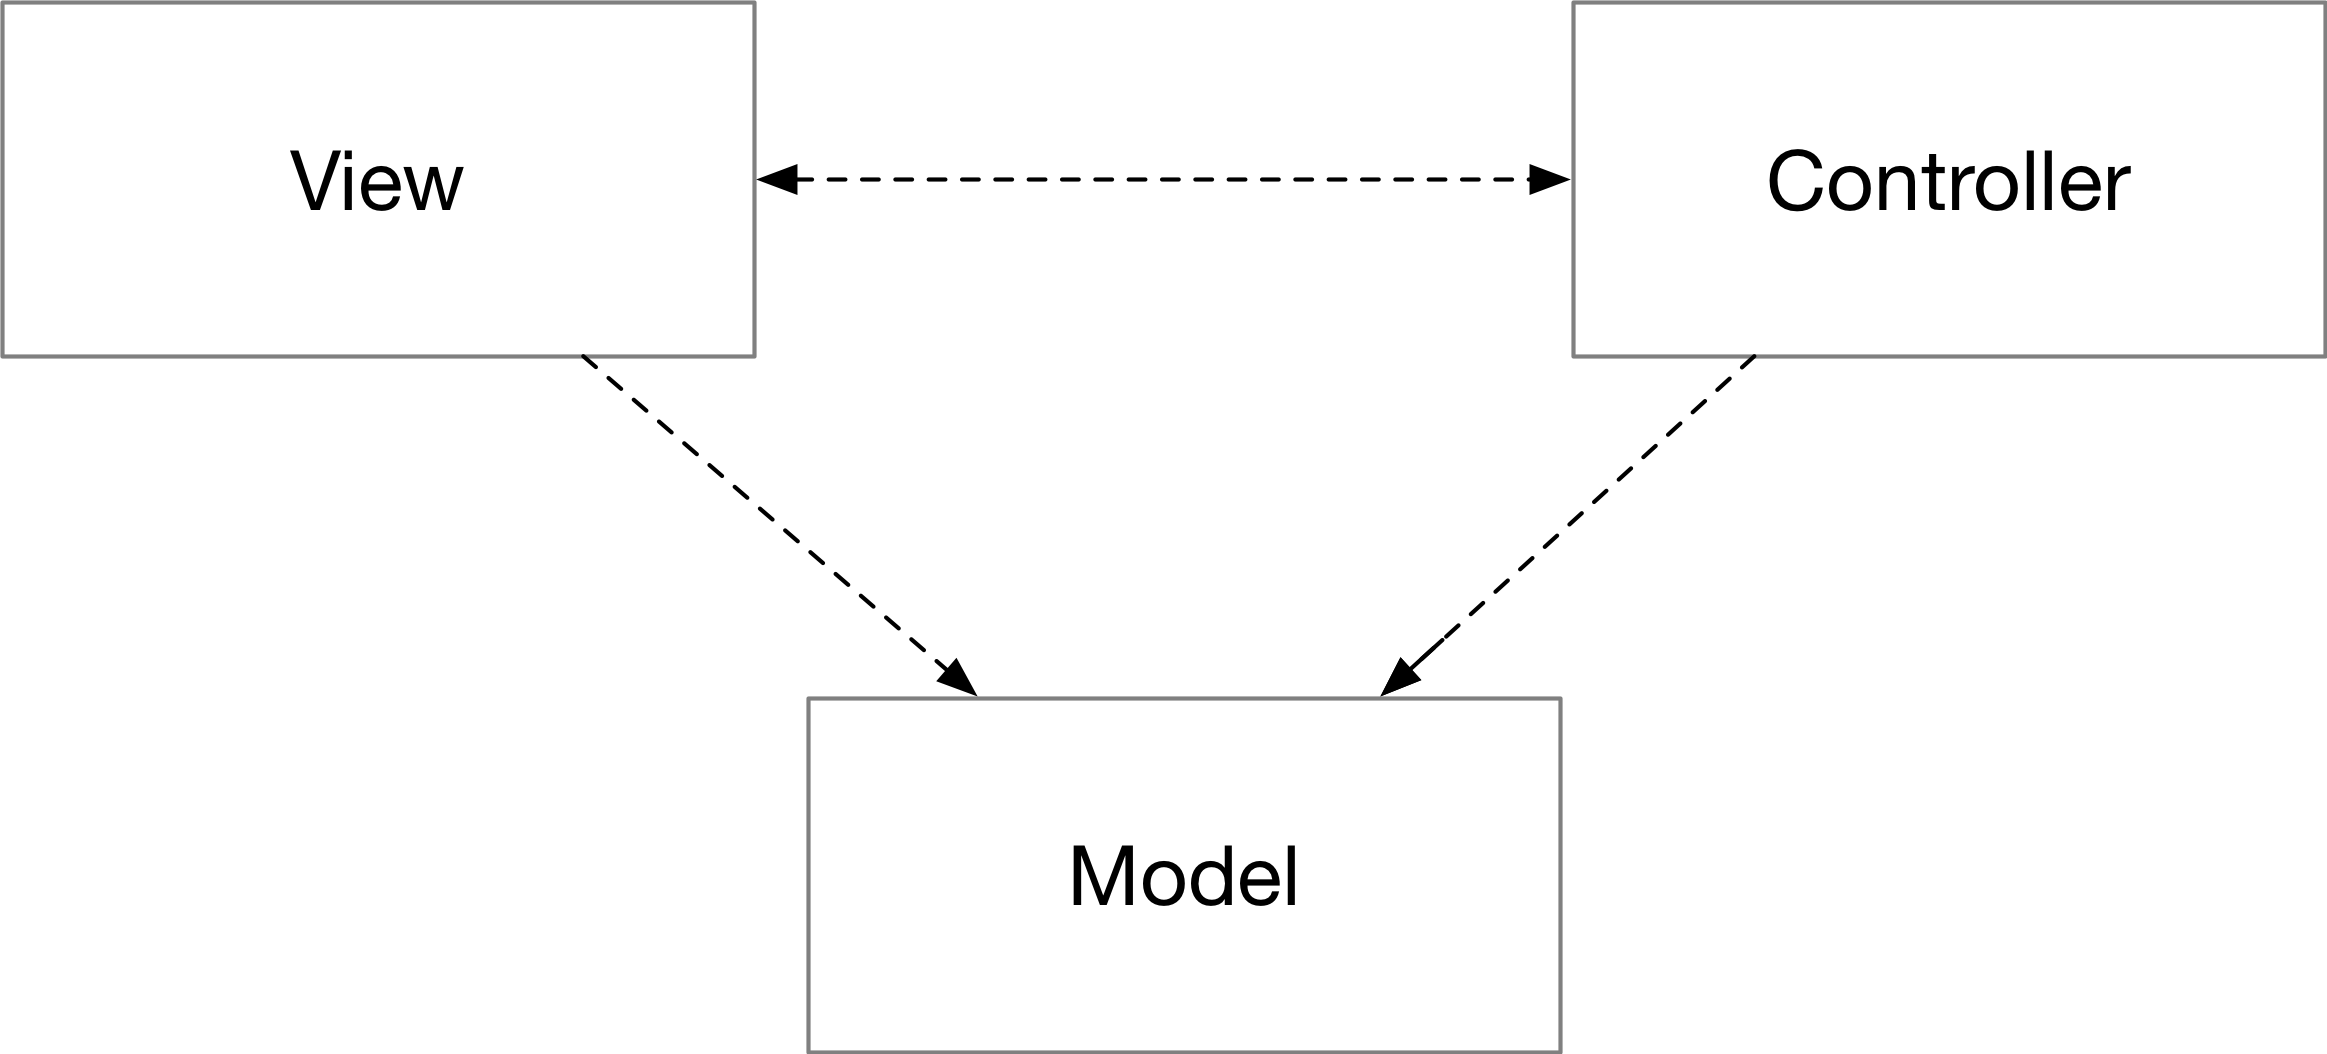
\includegraphics[scale=0.8]{bilder/grundlagen/MVC.png}
	\caption{MVC Pattern} source:\cite{GOLL}
	\label{fig:MVC}
\end{figure}


The so called separation of concerns makes it easier to split work and, due to that it makes it easier to maintain code. But it also comes with an increased complex setup process, changes for example in the model or the controller affect the whole entity. The bidirectional communication in the MVC structure makes it hard to debug, changing one entity  causes a cascading effect across the codebase.

\begin{figure}[H]
	\centering
	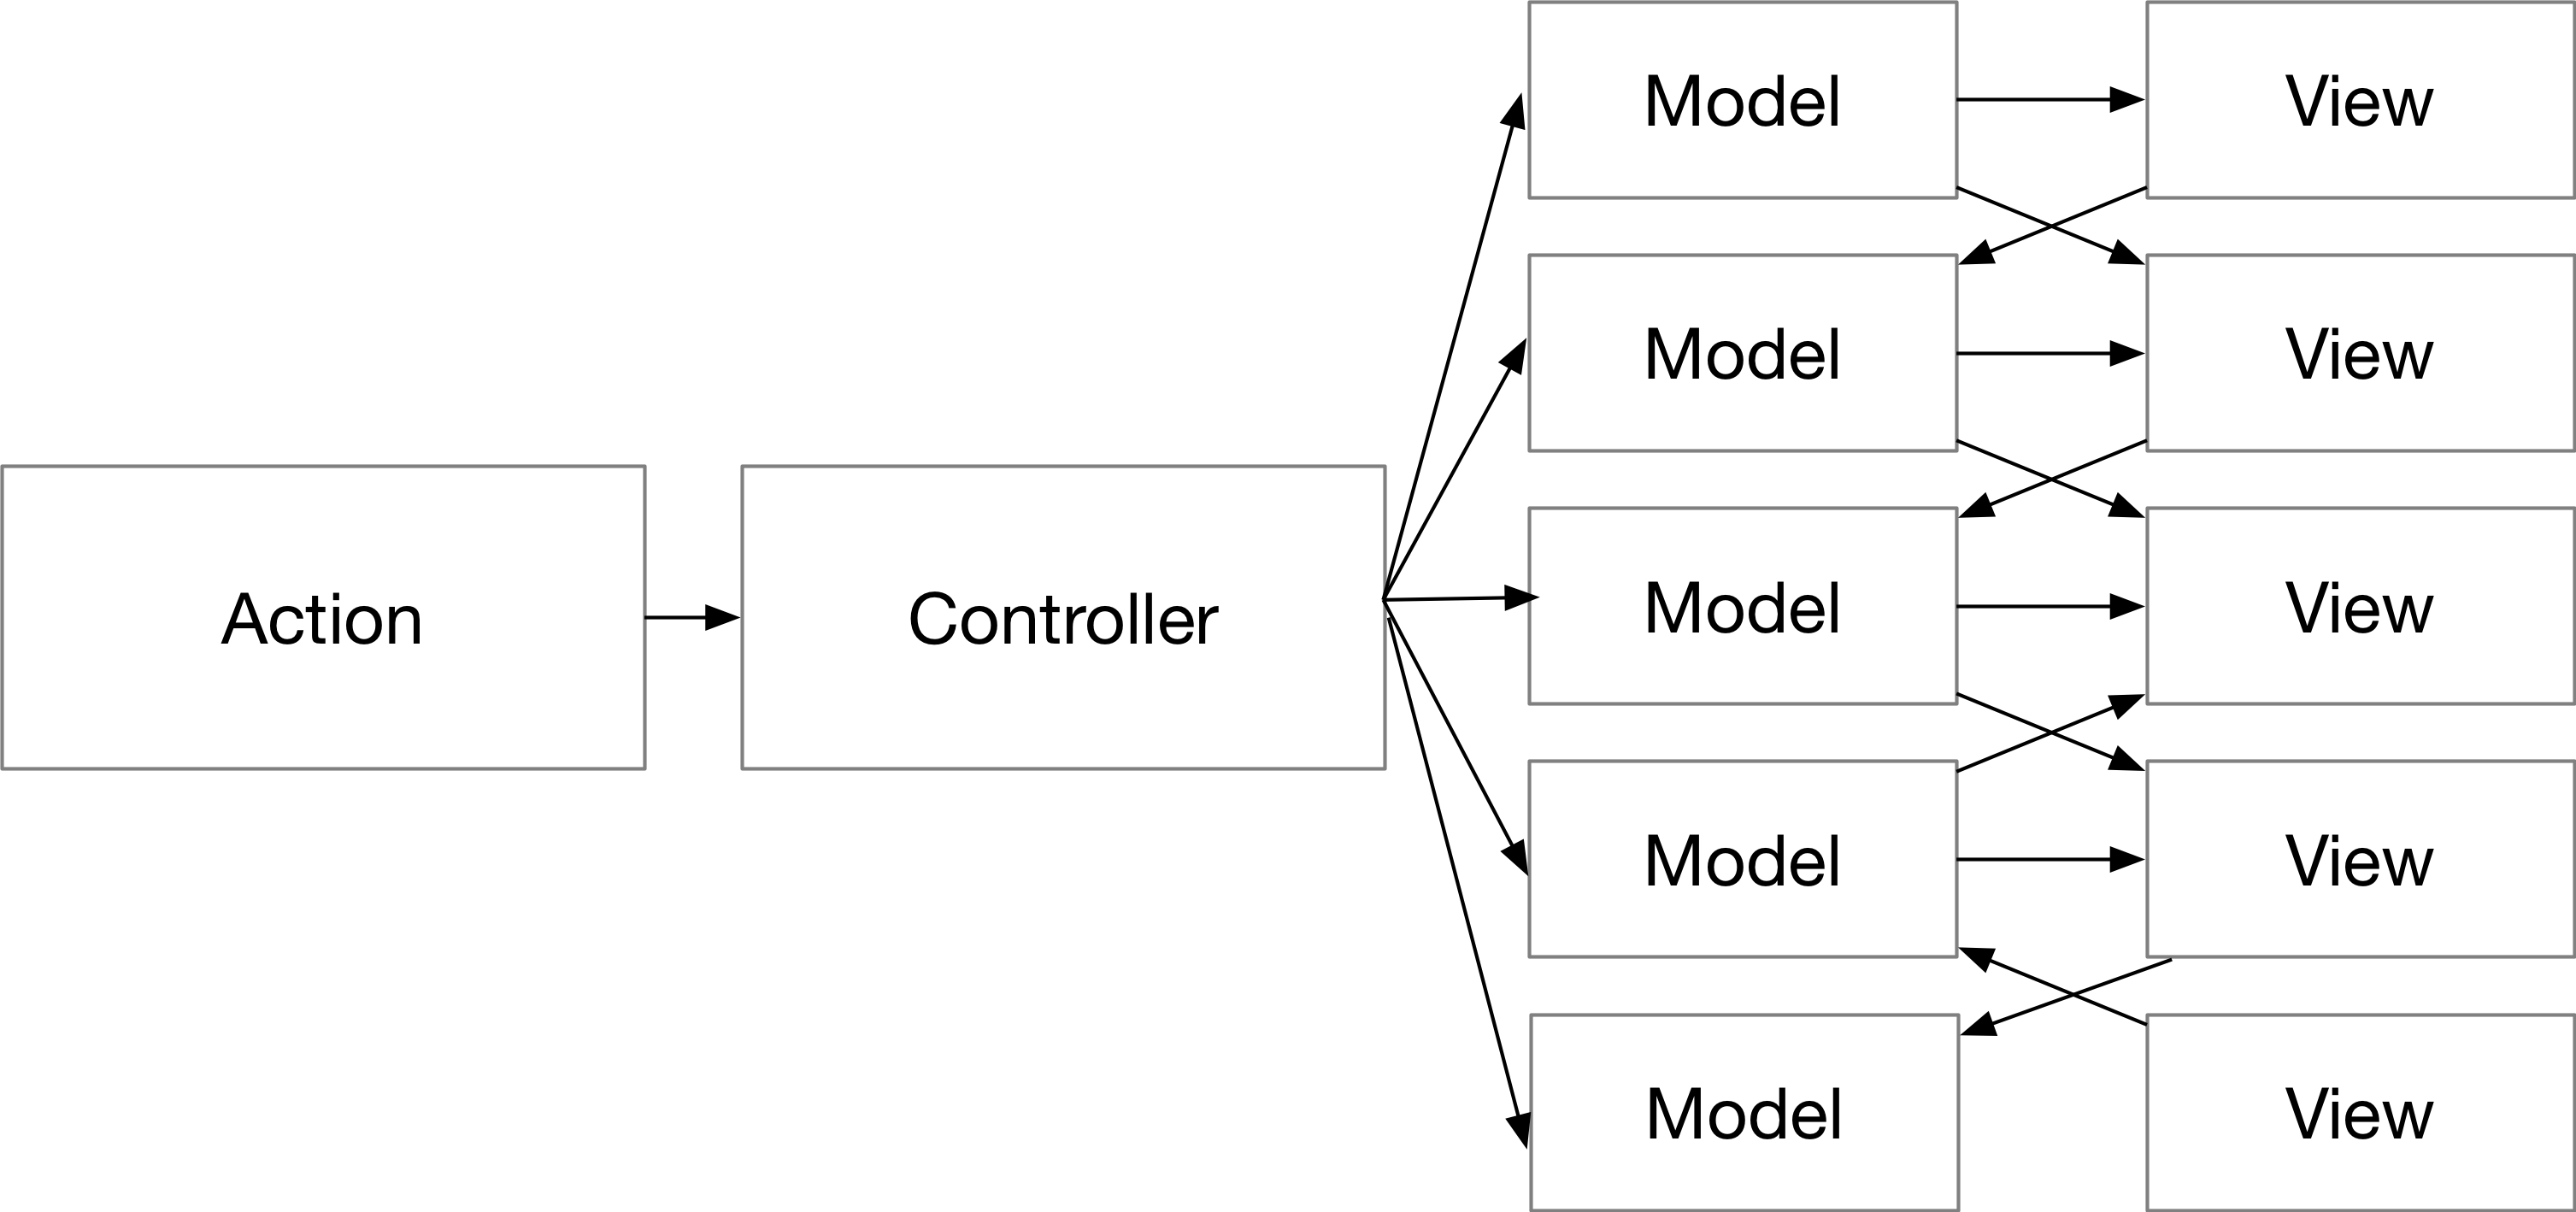
\includegraphics[scale=0.5]{bilder/grundlagen/mvcComplex.png}
	\caption{Complex MVC Exmaple} source:\cite{MVCExample}
	\label{fig:MVCExample}
\end{figure}
React tries to get rid of that by introducing a different architecture called Flux. The following section shall explain how Flux is different from the MVC pattern.

\subsection{Flux}

\subsubsection{Structure and Data Flow}

In Flux data flows in a single direction, the unidirectional data flow is central to Flux. Dispatcher, stores and views are independent nodes with different inputs and outputs. The actions simply consist of objects with the new data.


\begin{figure}[H]
	\centering
	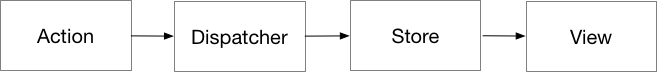
\includegraphics[scale=0.5]{bilder/grundlagen/uni.png}
	\caption{Flux Software Architecture} source:\cite{FLUX}
	\label{fig:FLUX}
\end{figure}

The dispatcher takes care of handling all actions and forwarding it to the right store. The store holds the data and actions to change this data. Once data was changed the store alerts all views that are affected by this data change, causing a re-rendering.

It is also possible that a view generates an action, this happens mainly through user interaction. This action is also passed to the dispatcher. 


\begin{figure}[H]
	\centering
	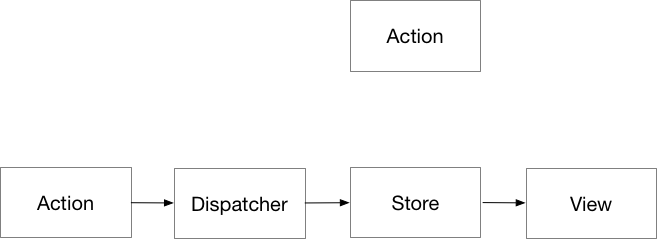
\includegraphics[scale=0.5]{bilder/grundlagen/uniDirection2.png}
	\caption{Flux with View Action} source:\cite{FluxAction}
	\label{fig:FA}
\end{figure}

\subsubsection{Dispatchers}
Dispatchers can be considered as a central hub that is managing all data flows in a Flux application.

The only way to change data, is through actions the dispatcher is providing.
A dispatcher has no real intelligence of its own, it only provides a simple mechanism to distribute action over several stores.

This becomes more important when big applications shall be built. The dispatcher then handles dependencies between different stores, he takes care of updating the different stores in a specific order.

\subsubsection{Stores}
Stores contain the application's logic and sates. This role can be considered somehow similar to a model in the traditional MVC,the difference is that stores manage the data of many objects and not a single record of data like ORM models do. They manage the application state for a whole domain. 

For example Facebook's Lookback Video Editor utilized a TimeStore that kept track of the playback time position and the playback state. On the other hand, the same application's ImageStore kept track of a collection of images.

\subsubsection{Views and Conroller-Views}

In React all views are composable and freely re-renderable. at the top of each view, the highest in hierarchy, there is a view that listens to events that are sent by the store. It is called a controller-view. 

The controller-view fetches the data from store and passes it down to all descendants, causing a re-rendering of that views. Often the entire state of a store is passed down a chain of views allowing each descendant to take what he needs.

\subsubsection{Actions}
As already mentioned action change the store . Each action has payload with new data, every time an action occurs a dispatch is triggered to the stores.
User-interaction is not the only of actions, it can also come from other places like the server.


\subsubsection{Conclusion}
The Flux architecture is improving data consistency, it offers better possibilities to debug. The unidirectional data flow makes that much easier. Since one can always follow the flow of actions.Furthermore with having the state and all the logic that is updatitng the state at one place  it is also possible to do more meaningful unit tests.

\section{React and Flux}
This section is about analyzing how React is implementing the Flux Software Architecture. React depends on encapsulated components that manage their own state. 

Components are written in JavaScript, so data can easily passed through the Application. Everything that needs to be rendered is still written in HTML and parsed by React. Each component has its own controllers, there is no more discrimination between what is shown in the Browser and business logic.

There are no separated HTML and JavaScript files, only JavaScript. Every component is fully standalone and testable by its own. This makes React scalable and easy to test. There are no cascading dependencies. Every time the state of a component changes, the render function is called and the HTML is re-rendered with the changed data. Components can be nested, e.g. a board game that consists of squares.

\begin{figure}[H]
	\centering
	\includegraphics[width=0.8 \textwidth]{bilder/grundlagen/Component.png}
	\caption{Component} source:\cite{Component}
	\label{fig:COMPONENT}
\end{figure}


Each of that squares is a component and part of the whole board game application. There shall bee a value assigned to the squares, values are passed through the prop value.

\begin{figure}[H]
	\centering
	\includegraphics[width=0.8 \textwidth]{bilder/grundlagen/Component2.png}
	\caption{Component} source:\cite{Component}
	\label{fig:COMPONENT}
\end{figure}



\begin{figure}[H]
	\centering
	\includegraphics[scale=0.5]{bilder/grundlagen/Component3.png}
	\caption{Component} source:\cite{Component}
	\label{fig:COMPONENT}
\end{figure}

Now when clicked on a square, this square shall show the 'X'. The value can now be considered a local state, it is definitely a private part of the square. First an initial state needs to be added.

\begin{figure}[H]
	\centering
	\includegraphics[width= \textwidth]{bilder/grundlagen/Component4.png}
	\caption{Component} source:\cite{Component}
	\label{fig:COMPONENT}
\end{figure}

If this.setState is called, an update is scheduled by React and the value is merged in the correct component state. Furthermore the component and all of its descendants are re-rendered. If a Square was clicked it would now show a 'X' in the grid.

\subsubsection{Lifting State Up}
Often data needs to be aggregated from multiple child components. Then it makes sense to lift all states up to the parent component. The parent component then passes down the individual states for the child components.

E.g. in a Tic Tac Toe game, to determine who has won, the value of all square components would need to be checked. That is technically doable but a better approach is to save all states in the parent component and the parent component can simply check one array in order to determine who has won. 

The Square component is no longer keeping its own state, it receives the value from its parent Board. It informs the parent when it was clicked. These components are called controlled components. 



\lstinputlisting{bilder/grundlagen/LiftingStateUp.js}


\begin{figure}[H]
	\centering
	\includegraphics[width=0.7 \textwidth]{bilder/grundlagen/Component5.png}
	\caption{Component} source:\cite{Component}
	\label{fig:COMPONENT}
\end{figure}


\subsubsection{Virtual DOM}

Manipulating the DOM is the main thing modern, interactive web applications do. Unfortunately it is a lot slower than running JavaScript. The HTML DOM is always tree structured, which makes it easy to traverse through it, but it also offers poor performance.

Additionally some modern frameworks update the DOM more often than it needs to be updated. For example changing one item in a list of ten items would lead to re-rendering all ten items. React is addressing this problem by introducing a virtual DOM.

The Virtual DOM is an exact representation of the HTML DOM with JavaScript. Once states have changed the virtual DOM is updated first, then the previous Virtual DOM is compared to the current Virtual DOM. Only what is different will be updated in the HTML DOM.

\begin{figure}[H]
	\centering
	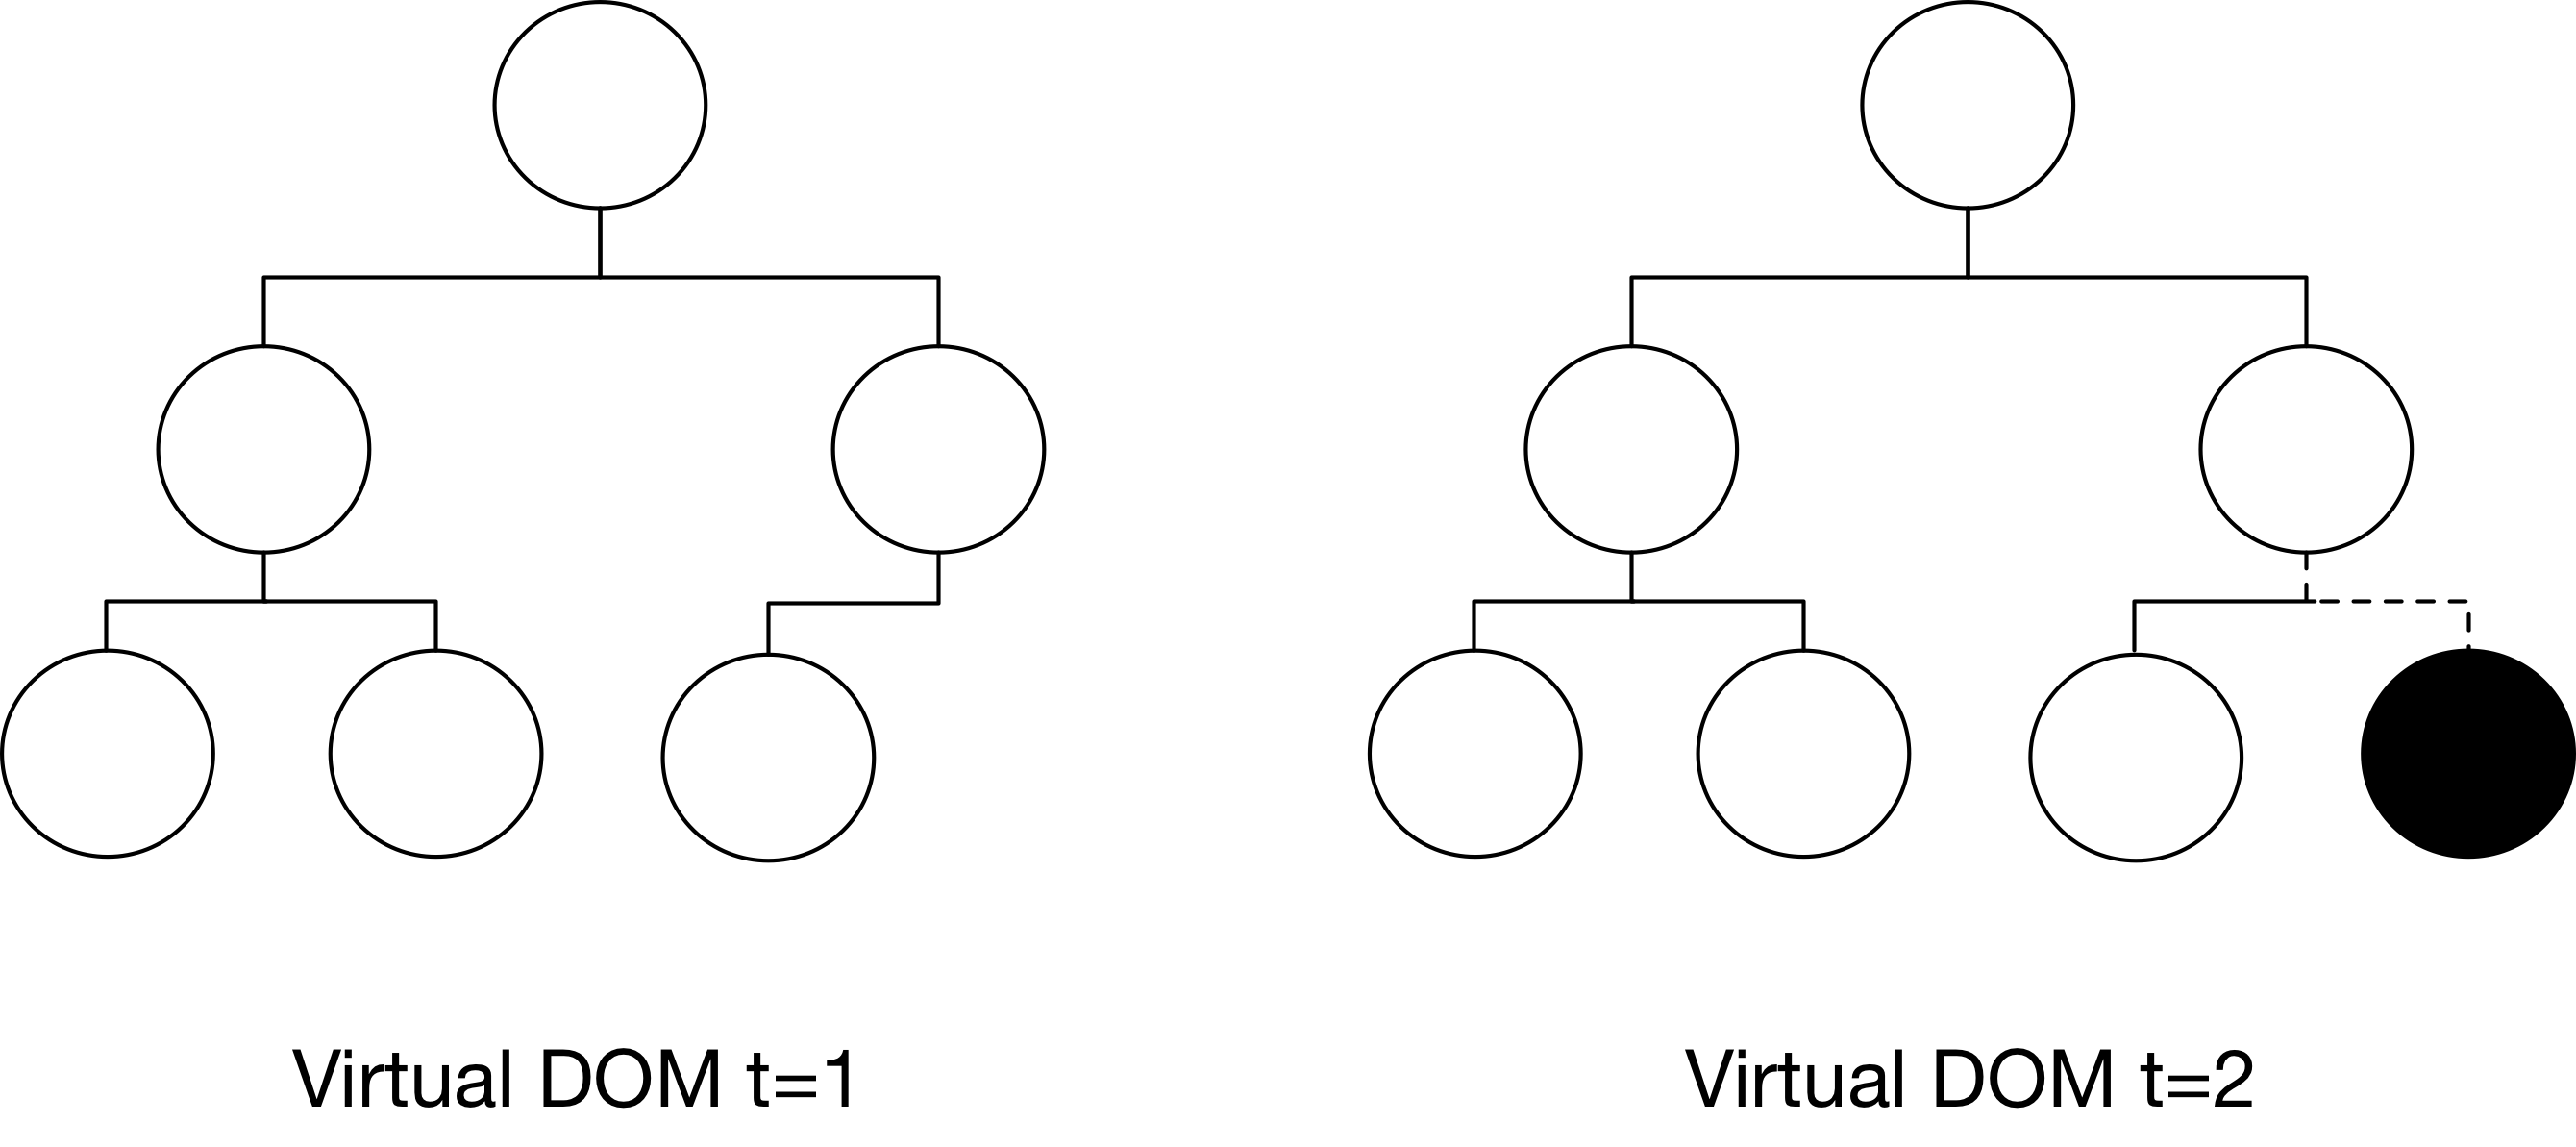
\includegraphics[width=0.7 \textwidth]{bilder/grundlagen/VirtualDom.png}
	\caption{Virtual DOM Camparison} source:\cite{Component}
	\label{fig:COMPONENT}
\end{figure}

\newpage

\subsubsection{Redux}
Redux is a predictable state container for JavaScript apps. It makes applications more consistent, by organizing all states in your app. Redux evolves the ideas of the Flux software architecture.
 
The gist of Redux is that all states are kept as an object tree ,in a single store. It is only possible to change this object tree by emitting an action, this action is an object describing what happened. To specify how these actions change the state tree, pure reducers are written.

The only difference to Flux is that Redux does not have a Dispatcher or support many stores. There is just a single store with a single root reducer. In bigger applications the root reducer can be split into smaller reducers, each operating independently on the different parts of the state tree. 

Redux adds a lot of overhead to an application, a lot of more files and code are created. Considering that Redux should only be used if the following points are true. 

\begin{itemize}
\item Reasonable amounts if data is changing over time
\item A single source of truth is needed
\item Keeping all of the states in a top-level component is no longer sufficient.
\end{itemize}




\begin{figure}[H]
	\centering
	\includegraphics[width=0.8 \textwidth]{bilder/grundlagen/Redux.png}
	\caption{Virtual DOM Camparison} source:\cite{Component}
	\label{fig:COMPONENT}
\end{figure}


\section{TensorFlow.js}






